% Template for PLoS
% Version 1.0 January 2009
%
% To compile to pdf, run:
% latex plos.template
% bibtex plos.template
% latex plos.template
% latex plos.template
% dvipdf plos.template

\documentclass[10pt]{article}

% amsmath package, useful for mathematical formulas
\usepackage{amsmath}
% amssymb package, useful for mathematical symbols
\usepackage{amssymb}

% graphicx package, useful for including eps and pdf graphics
% include graphics with the command \includegraphics
\usepackage{graphicx}
\usepackage[utf8]{inputenc}
\usepackage[T1]{fontenc}
\usepackage[icelandic,english]{babel}
\usepackage{float}

% cite package, to clean up citations in the main text. Do not remove.
\usepackage{cite}

\usepackage{color} 

% Use doublespacing - comment out for single spacing
%\usepackage{setspace} 
%\doublespacing


% Text layout
\topmargin 0.0cm
\oddsidemargin 0.5cm
\evensidemargin 0.5cm
\textwidth 16cm 
\textheight 21cm

% Bold the 'Figure #' in the caption and separate it with a period
% Captions will be left justified
\usepackage[labelfont=bf,labelsep=period,justification=raggedright]{caption}

% Use the PLoS provided bibtex style
\bibliographystyle{plos2009}

% Remove brackets from numbering in List of References
\makeatletter
\renewcommand{\@biblabel}[1]{\quad#1.}
\makeatother


% Leave date blank
\date{}

\pagestyle{myheadings}
%% ** EDIT HERE **


%% ** EDIT HERE **
%% PLEASE INCLUDE ALL MACROS BELOW

%% END MACROS SECTION

\begin{document}

% Title must be 150 characters or less
\begin{flushleft}
{\Large
\textbf{Predictability in a highly stochastic system~: measles in small populations}
}
% Insert Author names, affiliations and corresponding author email.
\\
Q. Caudron$^{1,\ast}$, 
A. S. Mahmud$^{2}$, 
C. J. E. Metcalf$^{1,3}$,
M. Gottfre{\dh}sson$^{3,4,5}$,
C. Viboud$^{3}$,
A. D. Cliff$^{6}$,
B. T. Grenfell$^{1,3}$
\\
\bf{1} Department of Ecology and Evolutionary Biology, Princeton University, Princeton, NJ, USA
\\
\bf{2} Office of Population Research, Woodrow Wilson School of Public and International Affairs, Princeton University, Princeton, NJ, USA
\\
\bf{3} Fogarty International Center, National Institutes of Health, Bethesda, MD, USA
\\
\bf{4} Department of Medicine, Landsp\'{i}tali University Hospital, Reykjav\'{i}k, Iceland
\\
\bf{5} Faculty of Medicine, School of Health Sciences, University of Iceland, Reykjav\'{i}k, Iceland
\\
\bf{6} Department of Geography, University of Cambridge, Cambridge, UK
\\
$\ast$ E-mail: qcaudron@princeton.edu
\end{flushleft}













% Please keep the abstract between 250 and 300 words
\section*{Abstract}

A standard assumption in the modelling of epidemic dynamics is that the population of interest is well-mixed, and that no clusters of metapopulations exist. The well-known and oft-used SIR model, arguably the most important compartmental model in theoretical epidemiology, assumes that the disease being modelled is strongly immunising, directly transmitted, and has a well-defined period of infection, in addition to these population mixing assumptions. Childhood infections, such as measles, are prime examples of diseases that fit the SIR-like mechanism. These infections have been well studied for many systems with large, well-mixed populations with endemic infection. Here, we consider a setting where populations are small and isolated. The dynamics of infection are driven by stochastic extinction-recolonisation events, producing large, sudden, and short-lived epidemics before rapidly dying out from a lack of susceptible hosts. Using a TSIR model, we fit prevaccination measles incidence and demographic data in Bornholm, the Faroe Islands, and four districts of Iceland, between 1901 and 1965. The datasets for each of these countries suffers from different levels of data heterogeneity and sparsity. We explore the potential for prediction of this model~: given historical incidence data and up-to-date demographic information, and knowing that a new epidemic has just begun, can we predict how large it will be~? We show that, despite a lack of significant seasonality in the incidence of measles cases, and potentially severe heterogeneity at the population level, we are able to estimate the size of upcoming epidemics, conditioned on the first time step, to within reasonable confidence. Our results have potential implications for possible control measures for the early stages of new epidemics in small populations.













\section*{Introduction}

Measles is a highly contagious and strongly immunising infection of the respiratory system \cite{Anderson1991}. Due to its high transmissibility and the lifelong immunity procured by infection, its epidemiology is conditional on the birth of susceptible individuals. As such, the temporal dynamics of measles are typically strongly oscillatory, driven seasonally by the increased contact rate amongst young children during school periods \cite{London1973, Fine1982, Schenzle1984}, assuming the population is large enough to sustain the infection. The critical community size, defined as the size of a population required to sustain the disease at an endemic level, is estimated to be between 250,000 and 500,000 \cite{Bartlett1957, Black1966, Keeling1997}. In large populations, measles has been extensively studied, typically demonstrating biennial dynamics in developed countries prior to the introduction of vaccines \cite{Bolker1995, Grenfell1997}. These modelling efforts are typically based on a class of continuous-time systems of differential equations, such as the SIR and SEIR compartmental models. Mechanistically, these models provide a good description of the driving mechanisms behind infections such as measles, which have a well-defined infectious period, are directly transmitted, and yield lifelong immunity to those who recover from the infection \cite{Anderson1991}. SIR-like also models assume, however, a certain level of homogeneous mixing between individuals in the population. In many large-populations studies, such as in \cite{Bjornstad2002}, these assumptions hold reasonably well~: the populations are large and spatially compact enough to guarantee sufficient mixing within the population and to ensure that the disease remains endemic. 

In small populations, however, the dynamics of measles cases are different. Susceptible individuals accumulate when measles is absent; then, driven by stochastic recolonisation, an epidemic may sweep through a large fraction of the susceptible population very quickly, only to go extinct abruptly as susceptibles fall below there threshold required for spread. This results in very sharp, spiky epidemics, whose timing may be impossible to predict; they are described as Type III by Bartlett \cite{Bartlett1957}. Methods typically used in the analysis of time-series or in dynamical systems theory are not adapted to the study of temporal changes of measles incidence in such small populations. Nonetheless, scaling analysis in small populations has revealed that some level of predictability can be found within the statistics of epidemic size and duration distributions, despite the small number of epidemics observed in the recorded data \cite{Rhodes1996a, Rhodes1996b}.

A discrete-time adaptation of SIR-like models was developed by Finkenst\"{a}dt and Grenfell \cite{Finkenstadt2000}. The TSIR model is a simple and computationally inexpensive system of difference equations which can be parameterised against observed incidence time-series and birth data, and is able to estimate non-analytical, time-varying contact and transmission rates. It has been successfully used in the analysis of seasonal variation of measles in several systems with large populations \cite{Glass2003, Metcalf2010}. In addition, the model has been applied to small populations that demonstrate persistent, periodic dynamics due to strong coupling with nearby large populations \cite{Grenfell2002, Bjornstad2002}. 

However, little has been done on applying the TSIR model to subendemic populations with recurring and episodic outbreaks. Datasets on the incidence of diseases such as influenza and measles have been created from medical and parish records in small and isolated populations, where the disease dynamics are dominated by the stochastic importation of infected individuals. These datasets have been studied from the perspective of historical geography, where the occurrence and spatiotemporal spread of epidemics are explained by features of the landscape and of local populations \cite{Cliff1981, Cliff2000}. Despite the availability of these datasets, however, no inference methods have yet been applied to the problem of characterising the dynamics of disease spread in these unique systems.

In this paper, we address the question of predictability of measles epidemics in subendemic, isolated populations. First, we present data on the demographics and disease incidence in prevaccination-era Bornholm, the Faroe Islands, and four districts in Iceland. Then, we summarise the TSIR model and fit the parameters of the model to the data. After generating predictions for the evolution of each epidemic, we compare the mean predictions with the original time-series, and the predicted size of each observed epidemic. Finally, we discuss the factors which may influence the accuracy of predictions, and possible improvements to the data and methods used for improved results.














\section*{Methods}

\subsubsection*{Data}

Measles incidence data were obtained for Iceland, from 1901 to 1965, from \cite{Cliff1981}. This dataset consists of monthly figures for measles cases reported in 47 medical districts (\textit{l\ae knish\'{e}ra\dh{}}), originally sourced from \textit{Heilbrig\dh{}issk\'{y}rslur} (Public Health in Iceland). Medical districts, the basic reporting unit for disease data in Iceland, are composed of \textit{hreppar} (communes) that are roughly equivalent to English parishes or American townships. Major revisions to the boundaries of medical districts took place twice during the study period : in 1907 and 1932. Monthly incidence data for the Faroe Islands, from 1912 to 1965, were obtained from \cite{Cliff2000}; this data was originally sourced from \cite{Lancaster1990}. For Bornholm, monthly measles incidence data from 1925 to 1965 were acquired from \cite{Kingdom}.

Demographic data for Iceland were obtained from \cite{StatsIceland}. Annual data on population and number of live births for the entire country were taken from \cite{StatsIcelandBirths}. Decennial population data from 1901 to 1965, for 262 municipalities, were obtained from \cite{StatsIcelandPop}. Municipality borders changed from three to five times during the study period. In addition, many municipalities had missing data. Medical districts and municipalities were matched based on names. Several matched districts were discarded either due to missing population data, or lack of confidence in the matching of the geographical boundaries. With the data available, we were able to match four district-municipality pairs~: Akureyri, Reykjav\'{i}k, Hafnarfj\"{o}r\dh{}ur, and Vestmannaeyjar. It is worth noting that matched medical district--municipality pairs may not encompass the exact same area, but one may be a (potentially partial) subset of the other. 

Data on the demographics of the Faroe Islands were taken from the Statistical Yearbooks of Denmark published by Statistics Denmark \cite{StatsDenmark}, and from Statistics Faroe Islands \cite{StatsFaroe}. Annual data on population and births from 1901 to 1965 were found in aggregated form for all of the islands in the Faroe archipelago. 

Demographic data for Bornholm was collected from several publications from \cite{StatsDenmark}. Annual population data for Bornholm were obtained from \cite{StatsDenmarkPop}, which contains detailed statistical information collected by Statistics Denmark. Pre-1930 annual birth data were obtained from the \textit{\AE{}gteskaber, F\o{}dte og D\o{}de} (Marriages, Births and Death) available from \cite{StatsDenmarkBirths1}. Post-1930 annual birth data were obtained from \textit{Befolkningsudvikling og sundhedsforhold 1901-60} (Population, Development and Health 1901--1960), from \cite{StatsDenmarkBirths2}.

Figure \ref{figIncidence} shows the reported incidence for Bornholm, the Faroe Islands, and four districts of Iceland, and Table \ref{tableTau} presents the mean populations and birth rates over the study period. All data for this paper can be found online at \texttt{http://github.com/QCaudron/SmallPopTSIR}.










\subsubsection*{The TSIR model}

%For systems with small, heterogeneous populations, epidemic dynamics are driven by stochasticity in the timing of disease recolonisations and in population mixing. As such, dynamical models such as the well established SIR model are unable to adequately represent the underlying biological processes which dictate the evolution of disease incidence over time.
The time-series SIR model \cite{Finkenstadt2000} is a discrete-time, stochastic model of disease progression written in terms of a set of difference equations. Assuming that the infection is fully immunising and that the infectious period is well-defined, then the evolution of the number of infected cases, $I$, can be written,
\begin{equation}
\mathbb{E}\left[I_{t+1}\right] = r_t \, S_t \, I_t^\alpha,
\label{TSIR_I}
\end{equation}
where $S_t$ is the number of susceptible individuals at time $t$, seasonal contact rates are represented by the periodic parameter $r_t = r_{t+P}$ for $P$ time steps per year, $0 < \alpha < 1$ allows for nonlinearities due to the discrete-time approximation and in nonhomogeneous mixing, and where $\mathbb{E}\left[\,\cdot\,\right]$ denotes the expectation operator. The time step is set as the generation time of the infection. Then, the number of susceptible individuals is defined by,
\begin{equation}
S_{t+1} = S_t + B_{t-d} - I_t + u_t, \quad \mathbb{E}\left[u_t\right] = 0.
\label{TSIR_S}
\end{equation}
Here, $u_t$ is  zero-mean additive noise. $B_{t-d}$ is the number of births born $d$ time step prior to $t$, the delay $d$ assumed due to maternal immunity, and set at four months \cite{Anderson1991}.

The observed number of cases, $C_t$, is assumed to be underreported by a reciprocal reporting rate $\rho_t \ge 1$, such that the true number of infected cases at time $t$ is given by $I_t = \rho_t \,C_t$. If the number of susceptible individuals $S_t$ fluctuates around a mean $\bar{S}$ such that $S_t = \bar{S} + Z_t$, then, from equation (\ref{TSIR_S}), the dynamics of the susceptible individuals around their mean $\bar{S}$ are given by
\begin{equation}
Z_{t+1} = B_{t-d} + Z_{t} - \rho_t\,C_t + u_t.
\label{iter}
\end{equation}
A major assumption made by the TSIR model is that all individuals will eventually become infected. As such, the incidence of infected cases should track births. Successive iteration of equation (\ref{iter}) yields,
\begin{equation}
Z_{t+1} = \sum_{i=1}^t B_{i-d} - \sum_{i=1}^t \rho_i \, C_i + \sum_{i=1}^t u_i + Z_0.
\label{sums}
\end{equation}
If $\rho_t = \rho$ is a constant, and $u_t$ is small, then equation (\ref{sums}) reflects a linear relationship between the cumulative births and the cumulative incidence. However, as $Z_{t+1}$ depends on $Z_t$, it can be shown that the reporting rate need not be a constant, and that it could be estimated using locally linear regression methods. Then, $Z_t$ can be found as the residuals of this regression. 






\subsubsection*{Fitting}

The time step in the difference equations (\ref{TSIR_I}) and (\ref{TSIR_S}) is fixed at the generation time of the infection. For measles, the period of time from infection to recovery is approximately two weeks \cite{Anderson1991}. Due to the very spiky nature of the reported incidence data (whose derivatives are non-smooth due to low sampling rates), interpolation must be done such that peaks in the data are not missed or reduced. As such, a linear interpolant with an integer multiple of the number of points per year was used. This yielded 24 time points per year, thus maintaining the maximum values of the peaks in the data, and fixing the generation time at just over fifteen days.

Population and live births, assumed to be smooth, were interpolated cubically. There are large intervals between some of the reported demographics data; however, Finkenst\"{a}dt and Grenfell \cite{Finkenstadt2000} report that the regression for reconstructing susceptibles is robust to pronounced changes in birth rates.

The reporting rate $\rho_t$ was estimated using Gaussian process regression, given the births and reported cases. Unlike splines or locally-weighted regression methods, Gaussian process regressions do not optimise smoothness of the fitted values, but instead honour the observed values in the data exactly, and yield the best linear unbiased predictions of values in between observations. Once found, $\rho_t$ is the derivative of the Gaussian process prediction for the cumulative number of births, with respect to the cumulative number of cases, and $Z_t$ are the residuals of the regression.

The mean number of susceptibles $\bar{S}$ was estimated marginally by profiling the likelihood of the logarithmic form of equation (\ref{TSIR_I}) :
\begin{equation}
\ln\big(\mathbb{E}\left[I_{t+1}\right]\big) = \ln(r_t) + \ln\left(\bar{S} + Z_t\right) + \alpha \ln\left(I_t\right),
\label{log}
\end{equation}
after which the seasonal contact rates $r_t$ were estimated conditionally on $\bar{S}$. The mixing parameter was fixed at $\alpha = 0.97$, as in \cite{Metcalf2010}, implying a small, nonlinear inhomogeneity, yet not significantly impacting transmission dynamics between large and small epidemics. 







\subsubsection*{Predictions}

Using the TSIR model as defined by the system of equations (\ref{TSIR_I}) and (\ref{TSIR_S}), predictions for epidemic dynamics were made by sampling the incidence $I_{t+1}$ from a negative binomial distribution~:
%I_{t+1} \sim \mathrm{Bin}\left(S_t, \, 1-\mathrm{e}^{-\,r_t\, I_t^\alpha}\right),
\begin{equation}
I_{t+1} \sim \mathrm{NB}\left(r_{t+1}\,S_t\,I_t^\alpha, \, I_t\right),
\end{equation}
with mean $\mathbb{E}\left[I_{t+1}\right] = r_{t+1} \, S_t \, I_t^\alpha$ and shape parameter $k = I_t$.

Due to the abundance of zeros in the incidence time-series, initial conditions cannot simply be taken as the point $\left(I_0, S_0\right)$. Instead, each epidemic must be simulated independently, with initial conditions given by the data at the time that the epidemic begins. For each epidemic, we fix the initial number of infected cases and susceptible individuals as per the observed data and the reconstructed susceptible time-series, respectively, and allow the simulation to continue until the next epidemic begins. Thus, we always simulate the same number of epidemics as given by the incidence data, where each epidemic is simulated given only the data available at the onset of that epidemic. 

In order to clearly establish the time of onset of an epidemic, a sensitivity threshold must be set. Let $\tau \in \mathbb{Z}^+$ define the number of reported infected cases necessary for any particular biweek period to be considered part of an epidemic. In order for epidemic detection to be robust, we convolve the incidence time-series with a nine-point Hanning window and round to the nearest integer; then, any biweeks where the smoothed series is greater than $\tau$ are to be counted as part of an epidemic. This ensures that points slightly under $\tau$ are not penalised, should the next few points be greater than $\tau$. This also reduces the risk of detecting sporadic recolonisations that fail to become full epidemics; it also ensures that, should an epidemic be occurring, but by chance, the first point of that epidemic is just below $\tau$, it is not ignored. 

A choice of $\tau = 1$ ensures that all available non-zero data is used. However, many potential epidemics go extinct before propagating through the population, especially in highly heterogeneous populations. As such, using $\tau=1$ would cause a number of strongly overestimated epidemics. We therefore treat $\tau$ as a sensitivity parameter, and fit it by selecting the sensitivity threshold which yields the highest correlation between the mean predicted epidemic traces and the incidence data, as defined by the coefficient of determination, $R^2$. Then, the first point in a sequence of time steps defined by this method as belonging to an epidemic is considered the onset of that epidemic.


















% Results and Discussion can be combined.
\section*{Results}

\subsubsection*{Dynamics}

After fitting parameters as described above, predicted epidemic time-series were generated for each of the six localities, using the sensitivity thresholds reported in Table \ref{tableTau}. The statistical fits, computed from the difference equations (\ref{TSIR_S}), (\ref{sums}), and (\ref{log}), illustrate a step-ahead prediction. The simulated time-series are generated from much sparser information, effectively using an $n$-step-ahead prediction, with $n$ representing the duration of an epidemic -- this is a better test of predictability of the final sizes of epidemics.

Figure \ref{figIncidence} shows the time-series of the number of reported and predicted cases in all six localities. Predictions are plotted as the mean incidence across ten thousand simulations, with their respective 95\% confidence intervals. High temporal synchronicity can be seen in the Icelandic localities. In general, epidemics in Iceland are of shorter duration, whilst those in Bornholm and the Faroe Islands are not quite as spiky. In all localities, epidemics seem to occur more frequently in the latter half of the time-series, perhaps due to an increase in birth rates after the baby boom. 

The reported coefficient of determination has been corrected by removing points where both the observed and predicted time-series are simultaneously zero, to reduce inflation of the coefficient due to the large number of zeroes in the time-series. Overall, good agreement is generally found with the observed data, with the highest correlation being in Hafnarfj\"{o}r\dh{}ur, a small district about ten kilometres from Reykjav\'{i}k. The worst fit is found in the Faroe Islands, by a significant margin; predictions here are characterised by a number of failed extinctions, general overestimation of epidemic sizes and durations, except for the single, large observed epidemic, which is significantly underestimated. It has been suggested that these very large epidemics may have fundamentally different dynamics \cite{Rhodes1996}, which would cause difficulties in parameter inference.

A number of predicted epidemics have a right shoulder, where the model predicts that epidemics take longer to go extinct than those observed. Depending on locality, many of these shoulders are small (Akureyri, Hafnarfj\"{o}r\dh{}ur, and Vestmannaeyjar). For other localities, predicted epidemics may fail to go extinct entirely, demonstrating cyclical behaviour until the beginning of the next epidemic (Bornholm, the Faroe Islands, and Reykjav\'{i}k). This may indicate that populations are strongly heterogeneous, and that the inhomogeneity parameter, fixed at $\alpha=0.97$ for these simulations, is an overestimate.

Inferred reporting rates and seasonal transmission rates are shown in Figure~\ref{figSims}. The inferred seasonalities have wide distributions, demonstrated by their large confidence intervals. This can be explained by the highly stochastic nature of measles recolonisations into their respective localities, which is the primary driver for when epidemics occur. This is in contrast to the seasonality inferred in studies of large populations, such as that of England and Wales in \cite{Finkenstadt2000}, where significant seasonal trends were found, and matched well with school-based contact times. When the transmission rates were fixed to a constant, such that $r_t = r \; \forall \; t$, neither the inferred parameters nor the predicted dynamics changed significantly. 






\subsubsection*{Predictability in Epidemic Sizes}

Rather than considering a point-wise comparison between the predicted and observed epidemic time-series, a potentially more robust measure of predictability is the total number of infected cases that a particular epidemic will generate. We define the size of an epidemic as the sum of reported cases $C_t$ for observed data, or $I_t / \rho_t$ for predicted data, from the first time point in an epidemic to the time point before the next epidemic begins. Figure~\ref{fig_sizes} shows the mean predicted epidemic size for each observed epidemic for the six localities. Several of these localities show a strong linear relationship, with near-zero intercepts and gradients around one. Again, the highest correlation between predicted and observed epidemic sizes is found in Hafnarfj\"{o}r\dh{}ur, with a coefficient of determination of $R^2 = 0.88$.







	 




























\section*{Discussion}

Predictions on epidemic sizes can be made with a significant level of certainty, despite sparse demographic data for all localities, mismatching incidence and demography information in Iceland, and strong spatial barriers to population mixing in the Faroe Islands. Hafnarfj\"{o}r\dh{}ur and Vestmannaeyjar show the best correlation between predicted and observed epidemic sizes, potentially due to their geography -- the former is a community just outside the capital city of Reykjav\'{i}k, small enough that district and municipality borders may match well; and the latter is a small island off the south coast of Iceland, with complementary demographic and incidence time-series. Perhaps for similar reasons of matching data streams and no major geographical restrictions to population mixing, Bornholm also shows a good correlation between expected and observed epidemic sizes. Epidemic sizes in both Akureyri and the Faroe Islands, however, are underestimated with respect to the observed epidemic sizes. For Akureyri, this could be due to an underestimation in the actual number of births in the area, caused by having a smaller municipality than the related medical district. This would generate a smaller reconstructed susceptible pool, reducing the sizes of predicted epidemics. For the Faroe Islands, the regression seems to be skewed to a smaller gradient by a single outlier whose size is grossly underestimated. Depending on the quality of the data, therefore, predictions about the size of a future epidemic can be made with some confidence. 

Data streams that do not represent exactly the same physical space, measurement, or system, are common problems in epidemiology and, indeed, in many fields where observation and data collection are non-trivial tasks, or where the system cannot be observed directly. Our results show the effects of data streams that do not quite match~: whether due to data aggregation in the Faroe Islands, or mismatching (and changing) borders for incidence and demographics data in Iceland, model fitting can be made more difficult. As an extreme case where data is abundant, and where demographic information is representative of the same regions as those of the measles incidence time-series, the TSIR model fitting performed by Finkenst\"{a}dt and Grenfell \cite{Finkenstadt2000} on sixty cities in England and Wales was highly successful.

Many improvements could be made to the dataset used in this paper to improve predictability of epidemic sizes. An understanding of where both the medical and municipal borders lie would allow a much larger number of districts to be fit confidently; in addition, an underlying spatial model could be used to counter the border changes and to analyse the data for spatial correlations. Disaggregated incidence and birth information for the large islands in the Faroe archipelago could be used to consider the separate island populations, each of which would have higher internal mixing, with a lower inter-island homogeneity. Noting that, in the second half of the Icelandic time-series, epidemics were perhaps becoming more regular, it may also be valuable to model the interepidemic intervals for longer time-series. 

With the current data, possible improvements include the use of statistical models such as trajectory matching or hidden Markov models to infer a biweekly incidence rate rather than using a linear interpolant, or the addition of an Exposed state variable to allow for exposed but not infectious individuals in a ``TSEIR'' model. 

Nonetheless, we have demonstrated that a strong signal of SIR-like epidemic dynamics can be found even in systems dominated by noisy importations. These well-known time-series \cite{Cliff1981, Cliff2000} are a paradigm for epidemics in small populations. Their sporadic nature is caused by long periods of time between stochastic importations followed by extinctions. As such, their dynamics are reminiscent of pandemics, where a significant proportion of the population is susceptible to infection at the onset of the epidemic. This interesting analogy extends to the lack of an observed seasonal signature. Our analysis reveals that, even from a highly stochastic incidence time-series and limited demographic data, reasonable predictions for the final size of an epidemic can be made, conditioned on the state of the system at epidemic onset. These results may have implications for the control of future epidemics, potentially informing response strategies based on the predicted size of an epidemic that was just initiated from a recolonisation event.

Significant spatial restrictions to population mixing, such as the fragmented island geography of the Faroe archipelago, may impact the level of predictability that can be found in these results. On the whole, however, we find that a homogeneous mass-action assumption is fairly successful overall -- with $\alpha \approx 1$, the model fits the data well for most localities. Indeed, Earn \textit{et al.} \cite{Earn2000} report that heterogeneous transmission is not required to obtain realistic dynamics in measles models. This is in contrast to the scaling analyses of Rhodes and Anderson \cite{Rhodes1996a, Rhodes1996b}, whose work suggests that heterogeneous dynamics are necessary to explain the distributions of final epidemic sizes and durations. Given the crudeness of the data, however, these results are tentative, and comparisons of our and their approaches are a fruitful area for future work.
























% Do NOT remove this, even if you are not including acknowledgments
\section*{Acknowledgements}

QC, CJEM, and BTG were supported by funding from the US Department of Homeland Security contract HSHQDC-12-C-00058. ASM acknowledges funding from the Eunice Kennedy Shriver National Institute of Child Health and Human Development (grant 5R24HD047879) and from the National Institutes of Health (training grant 5T32HD007163). BTG acknowledges support from the Bill \& Melinda Gates Foundation. CJEM and BTG were funded by the RAPIDD program of the Science and Technology Directorate, Department of Homeland Security, and the Fogarty International Center, National Institutes of Health. 








%\section*{References}
% The bibtex filename
\bibliography{qbib}

\section*{Figure Legends}
%\begin{figure}[!ht]
%\begin{center}
%%\includegraphics[width=4in]{figure_name.2.eps}
%\end{center}
%\caption{
%{\bf Bold the first sentence.}  Rest of figure 2  caption.  Caption 
%should be left justified, as specified by the options to the caption 
%package.
%}
%\label{Figure_label}
%\end{figure}


\section*{Tables}
%\begin{table}[!ht]
%\caption{
%\bf{Table title}}
%\begin{tabular}{|c|c|c|}
%table information
%\end{tabular}
%\begin{flushleft}Table caption
%\end{flushleft}
%\label{tab:label}
% \end{table}



\vspace{0.4cm}
\begin{table}[!h]
\centering
\begin{tabular}{ l c c c }
\hline \\[-0.9em]
\textbf{Locality} & Population & Birth rate & {$\mathbf{\tau}$} \\[0.1em]
  \hline \\[-0.9em]        
  Bornholm & 47100 & 19.4 & 15 \\[0.1em]
  Faroe Islands & 28200 & 29.4 & 15 \\[0.1em]
  Reykjav\'{i}k & 47100 & 24.1 & 18 \\[0.1em]
  Hafnarfj\"{o}r\dh{}ur & 6000 & 22.4 &  8 \\[0.1em]           
  Akureyri & 7000 & 22.7 & 19 \\[0.1em]
  Vestmannaeyjar \hspace{0.2cm} & 3600 & 23.5 & 7 \\[0.1em]
  \hline  
\end{tabular}
\caption{Mean population sizes, birth rates, and sensitivity thresholds $\tau$ for each locality. Population sizes and annual birth rates per thousand are given as the mean over the study period. Thresholds were fit by maximising the correlation between the mean simulated epidemic time-series and the reported incidence data.}
\label{tableTau}
\end{table}





\section*{Figures}

\begin{figure}[!h]
\centering
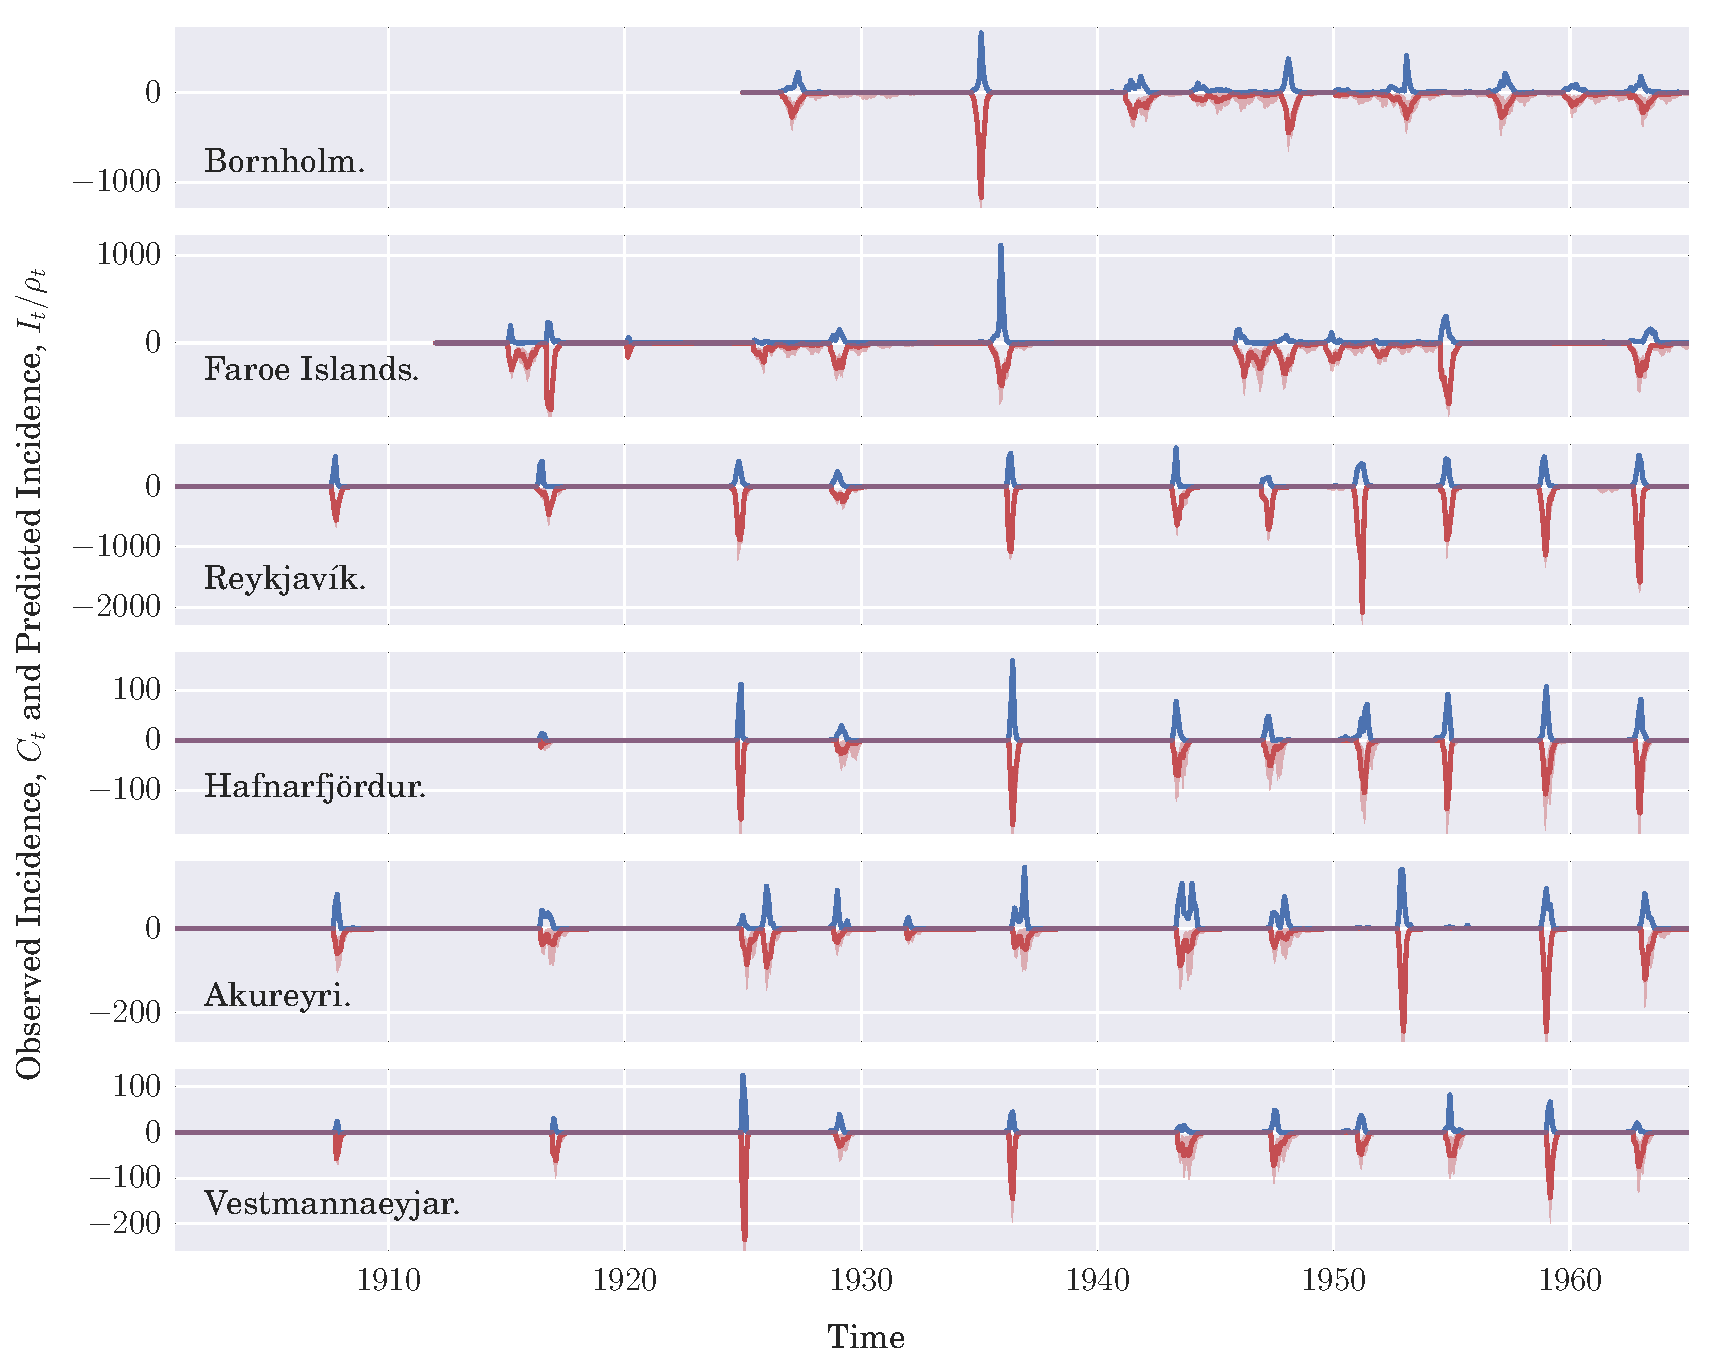
\includegraphics[width=\textwidth]{figures/q1.pdf}
\caption{\textbf{Reported and predicted biweekly incidence for Bornholm, the Faroe Islands, and four localities in Iceland.} The observed data is in blue. For the predicted time-series, the mean value of incidence simulations is plotted as a dark red line, with 95\% confidence intervals given in light red. Bornholm~: $R^2=0.78$; Faroe Islands~: $R^2=0.55$; Reykjav\'{i}k~: $R^2=0.73$; Hafnarfj\"{o}r\dh{}ur~: $R^2=0.86$; Akureyri~: $R^2=0.80$; Vestmannaeyjar~: $R^2=0.77$.}
\label{figIncidence}
\end{figure}



\begin{figure}[!h]
\centering
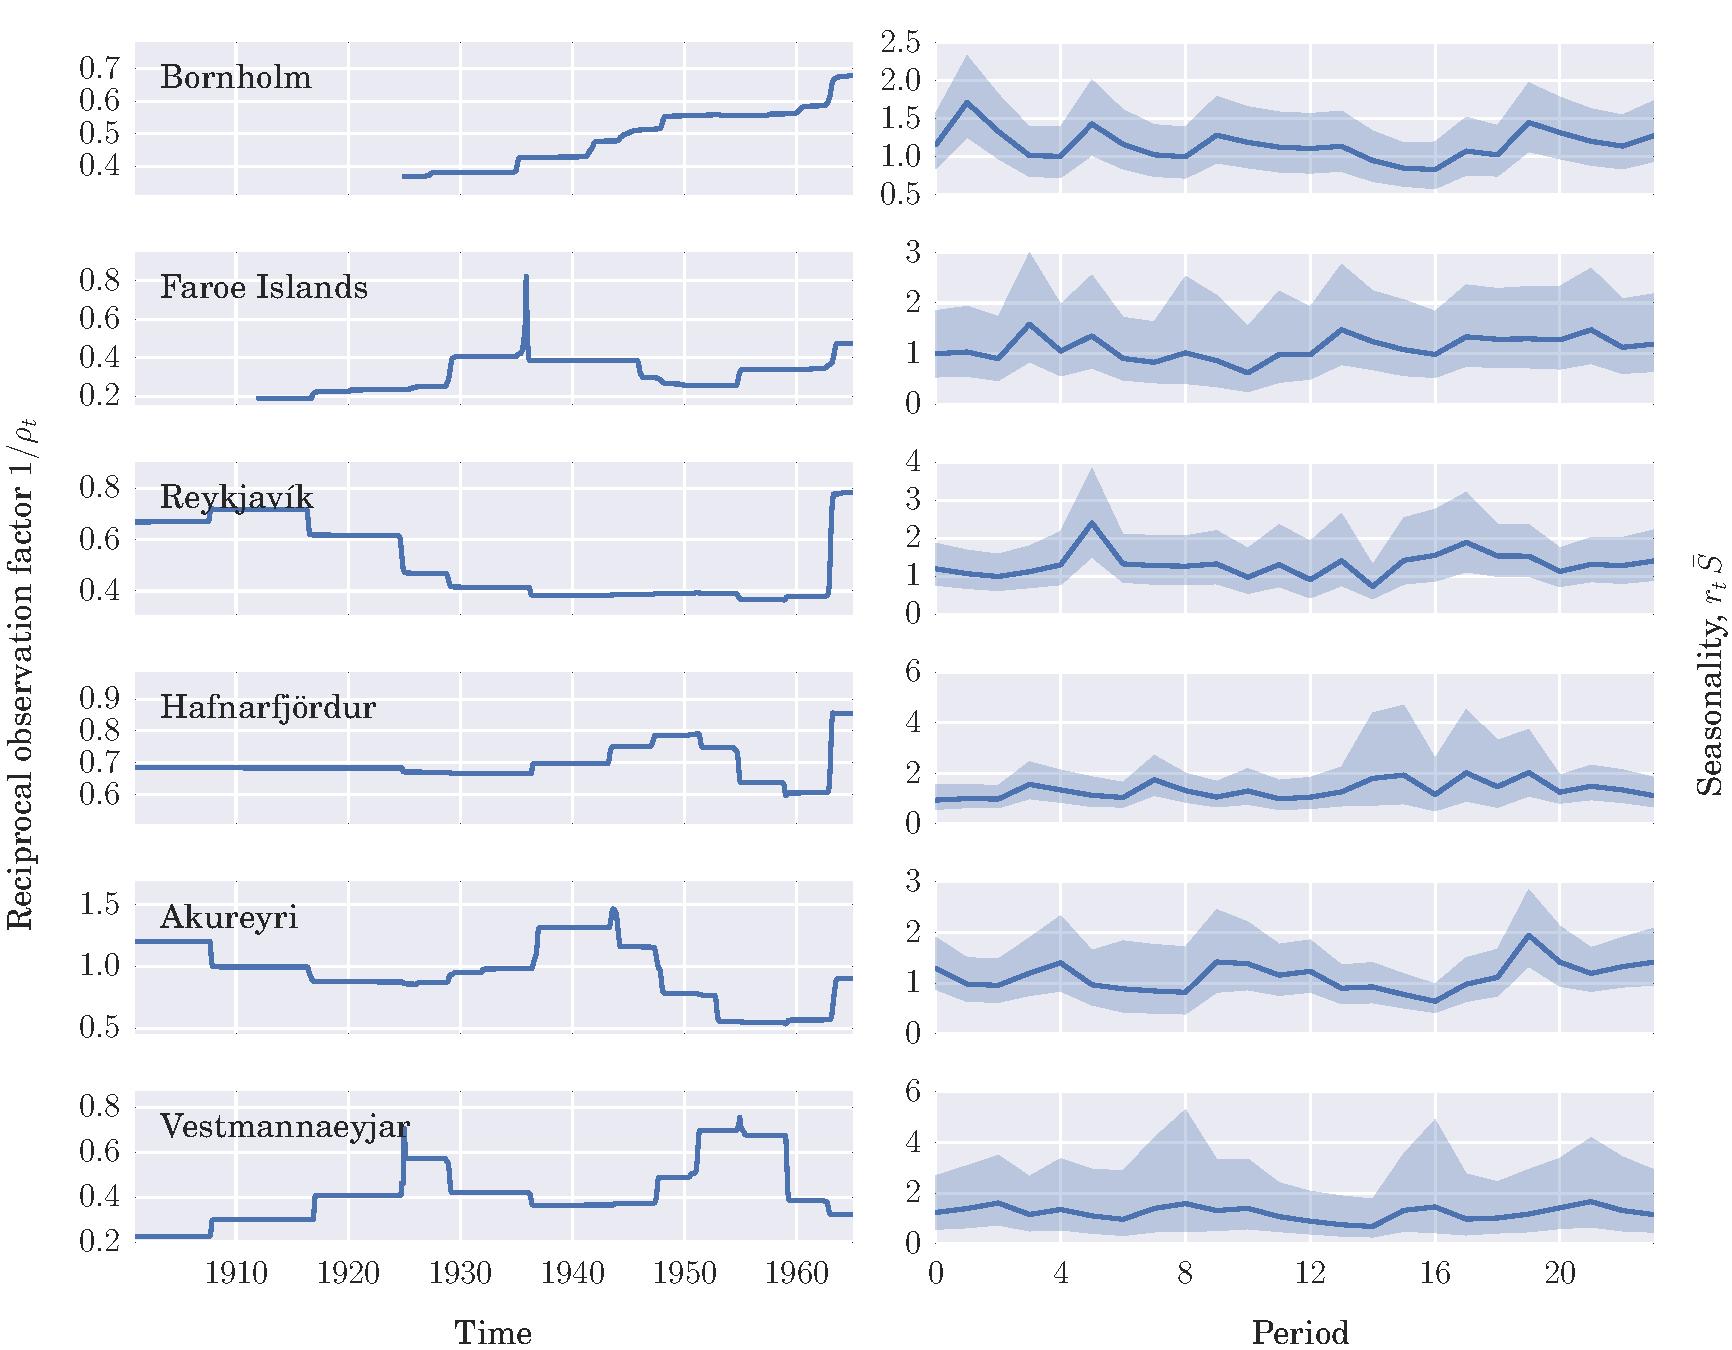
\includegraphics[width=\textwidth]{figures/q2.pdf}
\caption{\textbf{Reporting rates and seasonalities.} Seasonality is plotted as a function of the biweek, with 95\% confidence intervals in light blue.}
\label{figSims}
\end{figure}


\begin{figure}[!h]
\centering
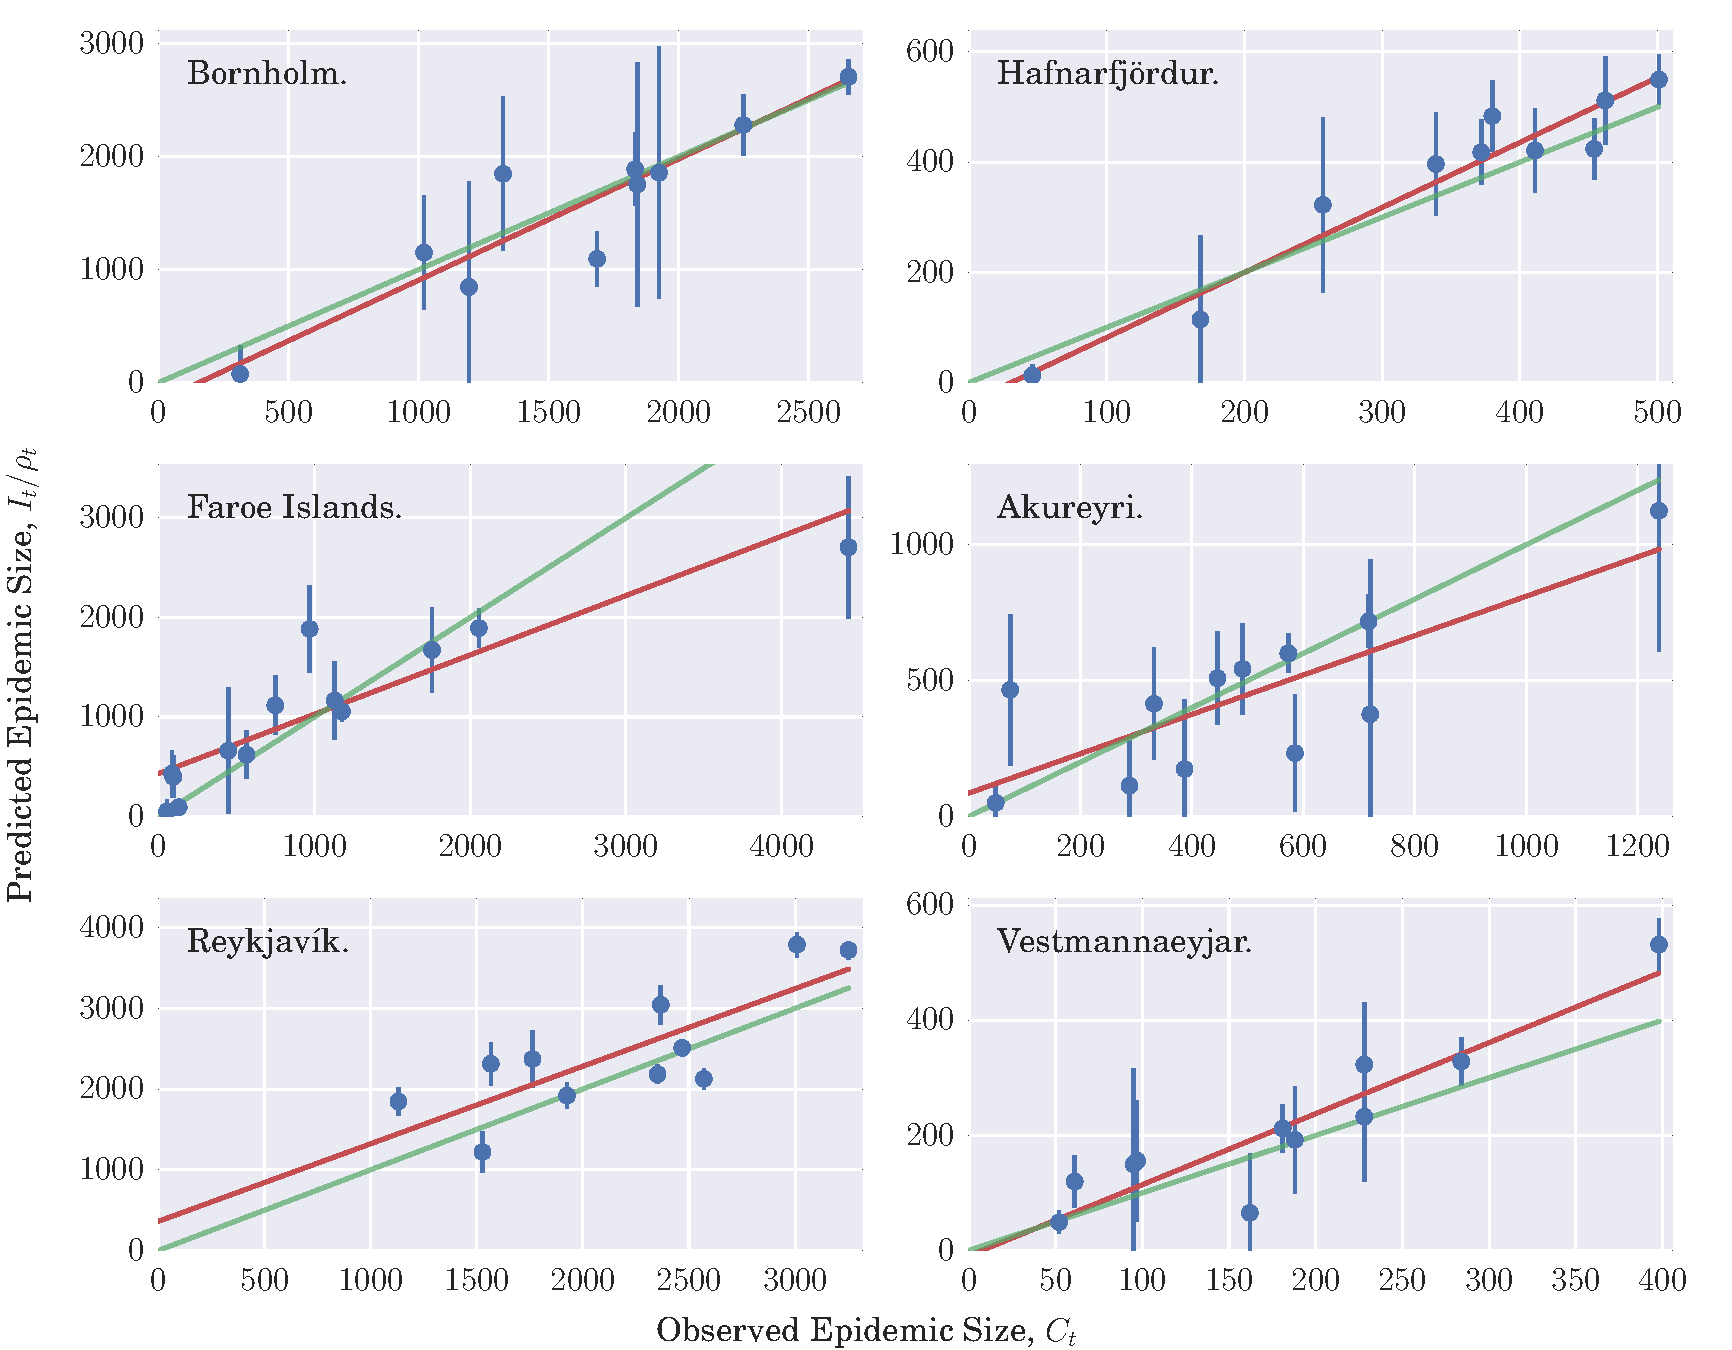
\includegraphics[width=\textwidth]{figures/q3.pdf}
\caption{\textbf{Predictability of epidemic sizes.} The mean predicted size of each epidemic as a function of its observed size, from ten thousand simulations. Red lines are the regression lines with the follow coefficients of determination and slopes~-- Bornholm~: $R^2=0.76$, gradient~$=1.07$; Faroe Islands~: $R^2=0.77$, gradient~$=0.60$; Reykjav\'{i}k~: $R^2=0.64$, gradient~$=0.96$; Hafnarfj\"{o}r\dh{}ur~: $R^2=0.88$, gradient~$=1.18$; Akureyri~: $R^2 = 0.49$, gradient~$=0.72$; Vestmannaeyjar~: $R^2=0.76$, gradient~$=1.23$. The green line is the zero-intercept, gradient-one line representing a one-to-one match between observation and prediction.}
\label{fig_sizes}
\end{figure}





\end{document}

